\chapter{Conclusions and further work}
\label{Kap5}

The last chapter of this Bachelor Thesis gives a brief summary of the developed software solution (see section \ref{conclusion}). In addition to that, some extension possibilities, like for example a new data model in order to connect the application to existing HIS, are described in section \ref{furtherwork}. 

\section{Conclusions} \label{conclusion}

As mentioned at the beginning of this chapter \ref{requirements}, the aim of this Bachelor Thesis is to improve logistics and the management of drugs in hospitals. By implementing a hybrid mobile application and connecting it to a MongoDB database, a very scalable as well as easy to use solution is purposed.
By implementing a real-time Socket.IO connection between clients and the database server medical staff can check the location and availability of drugs.
The given system offers a secure, approved solution to control the correct administration of drugs to each patient by checking the permission on the server-side. If a drug has been administrated successfully to a patient, it is not possible to repeat the administration. 
Moreover, using a 868 MHz frequency band drugs located on the same floor can be detected. To use the system, drugs need to be tagged with a RFID tag. 
In addition to that, the proposed solution replaces the paper-based administration of drugs to patients and prevents a duplicate administration of drugs or other errors.
Furthermore, the developed system has been established independently from any existing hospital information systems. Therefore, there is no preparation needed for the deployment in any department of hospitals.
To conclude, the given system can also be deployed in other contexts, like for example in schools or universities in order to check the attendance of students in exams (e.g. each student has a unique student's card which is tagged with a RFID tag).

\section{Further work} \label{furtherwork}

The developed application can be extended in many ways, that will be described next.

During testing in the HUCA, a nurse mentioned that when administering drugs to patients, she usually has to carry a medicine trolley with several containers, each for a specific patient. Actually, most of the patients in a hospital have to take more than only one drug which has to be organized in a list. In the past, the nurses had to manually check the patient related medication on a paper.
So, in future it would be very useful to divide the application into different sections which are related to a specific patient. This also implies, to change the format of the stored data. To be precisely, each patient could be stored in the MongoDB database as a top level document and contains various subdocuments which are his drugs. Since the structure of these drug documents already exists in the developed application, it would be very easy to adopt and implement that solution. Another possibility would be to connect the application to each electronic patient record, which can be seen in figure \ref{fig:newdatamodel}. Consequently, each patient can be easily identified with its medication list.

\begin{figure}
\centering
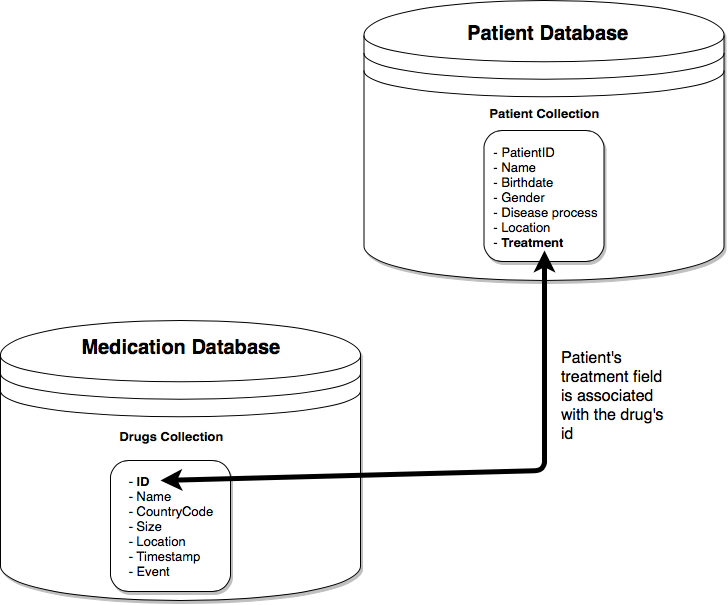
\includegraphics[width=\textwidth]{extension_mongodatamodel} 
\caption{\label{fig:newdatamodel}Example of extended data model, each patient entry is associated to the medication list} 
\end{figure}

Furthermore, in case of a patient's room where two or more patients are accomodated, the system should distinguish between those. To fastly identify a patient and its related medication on the medicine trolley, one solution could be to let patients wear a wristband with the same passive RFID tag as the drugs. Each time, the same antenna detects a drug and the patients wristband, it checks whether the drug should be administered to the patient and either allows the administration or not.

Another possible scenario would be to set up user roles in the application. This means, that for example the chief physician or the head of nurses sets up a list of medication related to each patient and only this person has access to the personal data. To provide patient's safety, there should be no other nurse or stuff in the hospital who can access the patient's related medication data. After setting up the drugs and its permissions to be administered to the specific patients, this "administrator" saves all data and logs out. 
Apart from this administrator, there will be another account, such as "nurse" or any ordinary user account. This person administers the drugs to each patients.